\documentclass[12pt,letterpaper]{article}
\usepackage{graphicx,textcomp}
\usepackage{natbib}
\usepackage{setspace}
\usepackage{fullpage}
\usepackage{color}
\usepackage[reqno]{amsmath}
\usepackage{amsthm}
\usepackage{fancyvrb}
\usepackage{amssymb,enumerate}
\usepackage[all]{xy}
\usepackage{endnotes}
\usepackage{lscape}
\newtheorem{com}{Comment}
\usepackage{float}
\usepackage{hyperref}
\newtheorem{lem} {Lemma}
\newtheorem{prop}{Proposition}
\newtheorem{thm}{Theorem}
\newtheorem{defn}{Definition}
\newtheorem{cor}{Corollary}
\newtheorem{obs}{Observation}
\usepackage[compact]{titlesec}
\usepackage{dcolumn}
\usepackage{tikz}
\usetikzlibrary{arrows}
\usepackage{multirow}
\usepackage{xcolor}
\newcolumntype{.}{D{.}{.}{-1}}
\newcolumntype{d}[1]{D{.}{.}{#1}}
\definecolor{light-gray}{gray}{0.65}
\usepackage{url}
\usepackage{listings}
\usepackage{color}

\definecolor{codegreen}{rgb}{0,0.6,0}
\definecolor{codegray}{rgb}{0.5,0.5,0.5}
\definecolor{codepurple}{rgb}{0.58,0,0.82}
\definecolor{backcolour}{rgb}{0.95,0.95,0.92}

\lstdefinestyle{mystyle}{
	backgroundcolor=\color{backcolour},   
	commentstyle=\color{codegreen},
	keywordstyle=\color{magenta},
	numberstyle=\tiny\color{codegray},
	stringstyle=\color{codepurple},
	basicstyle=\footnotesize,
	breakatwhitespace=false,         
	breaklines=true,                 
	captionpos=b,                    
	keepspaces=true,                 
	numbers=left,                    
	numbersep=5pt,                  
	showspaces=false,                
	showstringspaces=false,
	showtabs=false,                  
	tabsize=2
}
\lstset{style=mystyle}
\newcommand{\Sref}[1]{Section~\ref{#1}}
\newtheorem{hyp}{Hypothesis}

\title{Problem Set 3}
\date{Due: November 19, 2022}
\author{Tolga Bag - 23371290}


\begin{document}
	\maketitle
	\section*{Instructions}
	\begin{itemize}
		\item Please show your work! You may lose points by simply writing in the answer. If the problem requires you to execute commands in \texttt{R}, please include the code you used to get your answers. Please also include the \texttt{.R} file that contains your code. If you are not sure if work needs to be shown for a particular problem, please ask.
	\item Your homework should be submitted electronically on GitHub.
	\item This problem set is due before 23:59 on Sunday November 19, 2023. No late assignments will be accepted.

	\end{itemize}

		\vspace{.25cm}
	
\noindent In this problem set, you will run several regressions and create an add variable plot (see the lecture slides) in \texttt{R} using the \texttt{incumbents\_subset.csv} dataset. Include all of your code.

	\vspace{.5cm}
\section*{Question 1}
\vspace{.25cm}
\noindent We are interested in knowing how the difference in campaign spending between incumbent and challenger affects the incumbent's vote share. 
	\begin{enumerate}
		\item Run a regression where the outcome variable is \texttt{voteshare} and the explanatory variable is \texttt{difflog}.
		\vspace{0.2cm}
		\noindent I am checking the table and running the regression \\
		\lstinputlisting [language=R, firstline=39, lastline=42]{PS3.R} 
		\noindent voteshare is the dependent or outcome variable and difflog is the independent or explanatory variable. My null hypothesis is there is no relationship between voteshare and difflog. \\
		\lstinputlisting [language=R, firstline=46, lastline=46]{PS3.R} 
		\noindent p value is 0.0000000000000002, so I can reject the null hypothesis. Slope is 0.041666. In other words, for each unit change in difflog, voteshare is expected to increase by that amount. And it is a statistically significant result per the p value. \\
		\item Make a scatterplot of the two variables and add the regression line. 	\vspace{0.2cm}
		\lstinputlisting [language=R, firstline=52, lastline=61]{PS3.R} 
		\noindent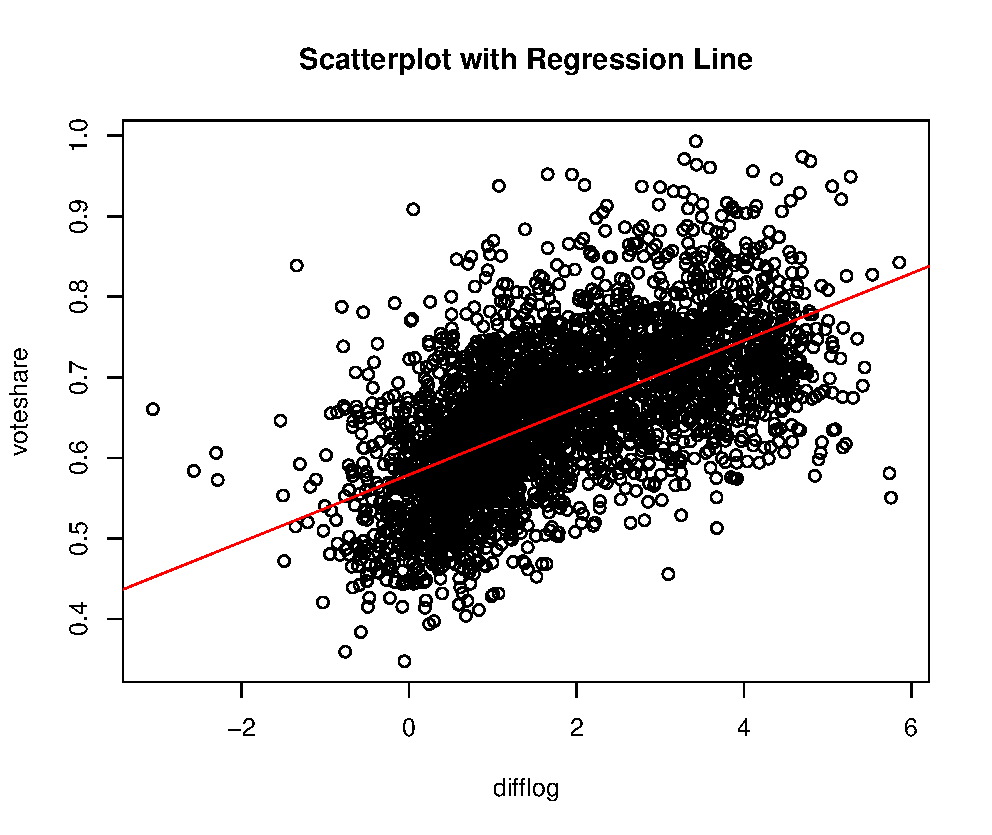
\includegraphics[width=.75\textwidth]{scatterplot1.pdf}
		\label{fig:scatterplot_1}
		\item Save the residuals of the model in a separate object.	\vspace{0.2cm}
		\lstinputlisting [language=R, firstline=64, lastline=66]{PS3.R} 
		\item Write the prediction equation.
		\lstinputlisting [language=R, firstline=69, lastline=83]{PS3.R} 
	\end{enumerate}

\section*{Question 2}
\noindent We are interested in knowing how the difference between incumbent and challenger's spending and the vote share of the presidential candidate of the incumbent's party are related.	\vspace{.25cm}
	\begin{enumerate}
		\item Run a regression where the outcome variable is \texttt{presvote} and the explanatory variable is \texttt{difflog}.	\vspace{0.2cm}
		\lstinputlisting [language=R, firstline=87, lastline=93]{PS3.R} 
		\item Make a scatterplot of the two variables and add the regression line. 	\vspace{0.2cm}
		\lstinputlisting [language=R, firstline=96, lastline=101]{PS3.R} 
		\noindent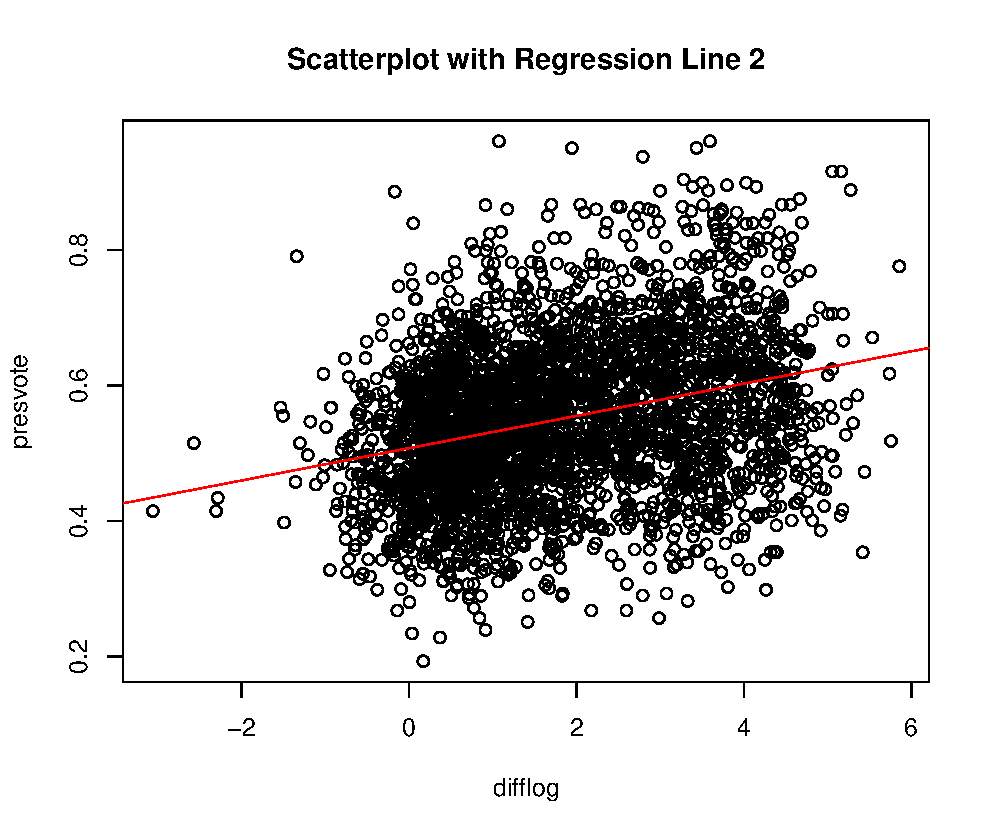
\includegraphics[width=.75\textwidth]{scatterplot2.pdf}
		\label{fig:scatterplot_2}
		\item Save the residuals of the model in a separate object.	\vspace{0.2cm}
		\lstinputlisting [language=R, firstline=105, lastline=106]{PS3.R} 
		\item Write the prediction equation.
		\lstinputlisting [language=R, firstline=109, lastline=120]{PS3.R} 
	\end{enumerate}
	
\section*{Question 3}

\noindent We are interested in knowing how the vote share of the presidential candidate of the incumbent's party is associated with the incumbent's electoral success.
	\vspace{.25cm}
	\begin{enumerate}
		\item Run a regression where the outcome variable is \texttt{voteshare} and the explanatory variable is \texttt{presvote}. \vspace{0.2cm}
		\lstinputlisting [language=R, firstline=125, lastline=126]{PS3.R} 
		\item Make a scatterplot of the two variables and add the regression line. \vspace{0.2cm}
		\lstinputlisting [language=R, firstline=129, lastline=133]{PS3.R} 
		\noindent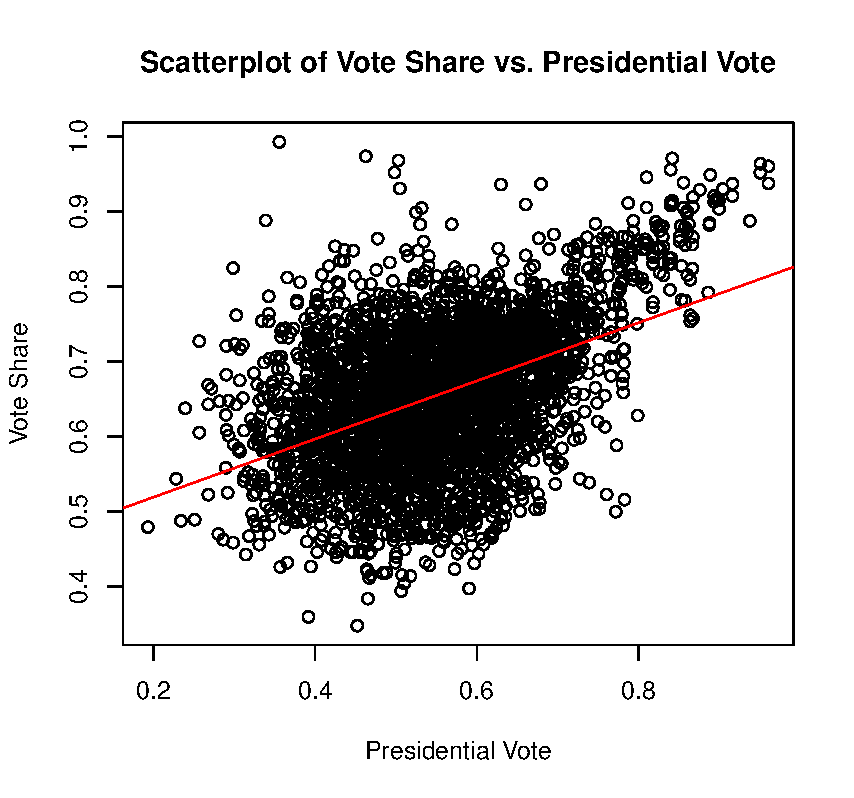
\includegraphics[width=.75\textwidth]{scatterplot3.pdf}
		\label{fig:scatterplot_3}
		\item Write the prediction equation.
		\lstinputlisting [language=R, firstline=136, lastline=146]{PS3.R} 
	\end{enumerate}

\newpage	
\section*{Question 4}
\noindent The residuals from part (a) tell us how much of the variation in \texttt{voteshare} is $not$ explained by the difference in spending between incumbent and challenger. The residuals in part (b) tell us how much of the variation in \texttt{presvote} is $not$ explained by the difference in spending between incumbent and challenger in the district.
	\begin{enumerate}
		\item Run a regression where the outcome variable is the residuals from Question 1 and the explanatory variable is the residuals from Question 2.	\vspace{0.2cm}
		\lstinputlisting [language=R, firstline=151, lastline=152]{PS3.R}
		\item Make a scatterplot of the two residuals and add the regression line. 	\vspace{0.2cm}
		\lstinputlisting [language=R, firstline=155, lastline=159]{PS3.R} 
		\noindent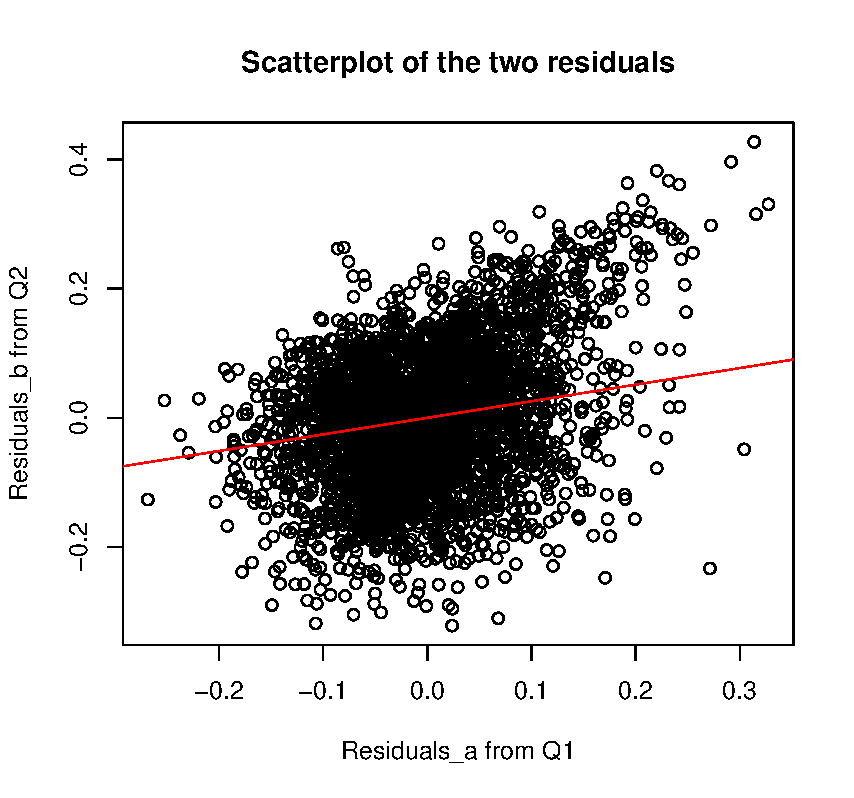
\includegraphics[width=.75\textwidth]{scatterplot4.pdf}
		\label{fig:scatterplot_4}
		\item Write the prediction equation.
		\lstinputlisting [language=R, firstline=162, lastline=72]{PS3.R} 
	\end{enumerate}
	

\section*{Question 5}
\noindent What if the incumbent's vote share is affected by both the president's popularity and the difference in spending between incumbent and challenger? 
	\begin{enumerate}
		\item Run a regression where the outcome variable is the incumbent's \texttt{voteshare} and the explanatory variables are \texttt{difflog} and \texttt{presvote}.	\vspace{0.2cm}
		\lstinputlisting [language=R, firstline=177, lastline=179]{PS3.R}
		\item Write the prediction equation.	\vspace{0.2cm}
		\lstinputlisting [language=R, firstline=182, lastline=196]{PS3.R}
		\item What is it in this output that is identical to the output in Question 4? Why do you think this is the case?
		\noindent The residuals are exactly the same. I think it is because both regressions are checking the effect of difflog. The one in Question 4 does it indirectly through the residuals of models that already accounted difflog, while the multi variate model does it directly. \\
	\end{enumerate}

\end{document}
